\chapter{Présentation du sujet}
Aboard Engineering est une entreprise spécialisée dans les domaines de
l'informatique embarquée. Les problématiques logicielles qu'elle rencontre sont
liées au matériel sur lequel sera déployé le code développé. Pour faciliter ce
type de développement, les concepteurs de logiciels embarqués se tournent de
plus en plus vers des outils de \gloss{mbd} qui permettent d'utiliser des langages
de haut niveau -- souvent graphiques -- pour la conception et la spécification
des systèmes à développer. On peut citer par exemple Matlab\up{\circledR}
Simulink\up{\circledR} qui est un outil permettant de définir graphiquement sous
forme de schéma logique le fonctionnement de systèmes complexes. C'est
d'ailleurs l'outil utilisé par Aboard Engineering pour définir ses fonctions de
contrôle moteur. Les avantages de ces modèles sont multiples. Premièrement, les
outils de MBD permettent de simuler l'exécution du système afin de
vérifier son fonctionnement. Ensuite, ces outils embarquent généralement un
générateur de code afin de générer le code correspondant à ces modèles,
allégeant grandement le travail des concepteurs et évitant au maximum les
erreurs faites lors de développement \og manuel\fg{}. En reprenant l'exemple de
Matlab\up{\circledR} Simulink\up{\circledR}, la suite intègre un générateur de
code embarqué temps réel appelé \gloss{rtw}. Il génère aujourd'hui le code des
prototypes de fonctions de contrôle moteur développés par l'équipe. J'y
reviendrai dans la section \ref{sec:rtw} plus en détail.

Comme dit précédemment, la génération de code facilite le travail de conception
et de réalisation de prototype. Cependant, pour pouvoir compiler le code de
plusieurs modules différents en une seule application, il reste des étapes à
réaliser. C'est ici que la plateforme de prototypage rapide Orianne
entre en jeu. Son rôle est de mettre en relation ces modules et de créer la
\og glue \fg{} entre tous les composants.\\
La plateforme Orianne est composée de plusieurs parties que nous appellerons \og
composants \fg{}. J'entrerai plus dans le détail dans la section \ref{sec:rtw}.

\section{La génération de code embarqué}
\subsection{État des lieux}
\label{sec:rtw}
Le développement d'une application pour un calculateur moteur est une tâche
complexe qui peut prendre un certains temps. De nombreux modèles sont
nécessaires à la spécification de tous
les aspects du fonctionnement d'un moteur ou des différentes commandes
utilisateur (pédales, boîte de vitesse, etc). À cela peut s'ajouter
la gestion d'une configuration hybride -- un moteur thermique couplé à un moteur
électrique -- nécessitant une gestion plus pointue de l'énergie.

Une fois complets, ces modèles ont vocation à être traduits en code source qui
sera compilé puis intégré dans un calculateur. C'est donc ce code compilé qui
est la base du contrôle moteur d'un véhicule. On comprend alors les contraintes
de fiabilité et de performance sous-jacentes.\\

Pour générer ce code, nous utilisons Matlab\up{\circledR} RTW-EC\up{\circledR}. C'est un
générateur de code embarqué temps réel puissant et reconnu pour fournir du code
suivant les normes en vigueur dans l'automobile.
Le code généré contient toute la logique métier et donc l'essentiel de la
complexité de l'application. Sur ce point, Matlab\up{\circledR} RTW-EC\up{\circledR}
fournit des résultats très bons en terme de temps d'exécution, de mémoire
utilisée ou de taille de pile lors des appels aux fonctions des modules.\\

Ce processus a l'air de fonctionner. Cependant, les contraintes budgétaires
sont également un point important à ne pas négliger. La suite Matlab\up{\circledR} coûte
très cher. Même pour une entreprise -- d'autant plus pour une entreprise de
petite taille comme Aboard Engineering --, les coût des licences
Matlab\up{\circledR} couvrant toute la suite nécessaire à l'ensemble du
processus de production sont significatif lors de la budgétisation d'un projet.\\

La problématique est alors de retrouver les même garanties de performance et de
qualité du code délivrées par Matlab\up{\circledR} sans le coût exorbitant
qu'engendre l'achat de licences. C'est pourquoi Aboard Enginnering a décidé de
se tourner vers une alternative libre : \gloss{qgen} et \gloss{projectp}.

\subsection{QGen}
A la base de QGen, on trouve un projet open source appelé
Project P (cf. figure \ref{fig:projectp}). Le but du projet P est de supporter le MBD pour des
système temps réel embarqués en fournissant un framework de génération de code
open source capable de :
\begin{enumerate}
  \item vérifier l'intégrité d'un point de vue sémantique de systèmes conçus avec
	différents langages de modélisation (Matlab\up{\circledR}
	Simuling\up{\circledR}, Scicos, Xcos, SysML, MARTE, UML) ;
  \item générer du code source optimisé pour des langages de programmation
	(Ada, C/C++) et des langages de synthèse (VHDL, SystemC) ;
  \item supporter des processus de certification de différents domaines
	(avionique, spatial, automobile).
\end{enumerate}

\begin{figure}[h]
  \centering
  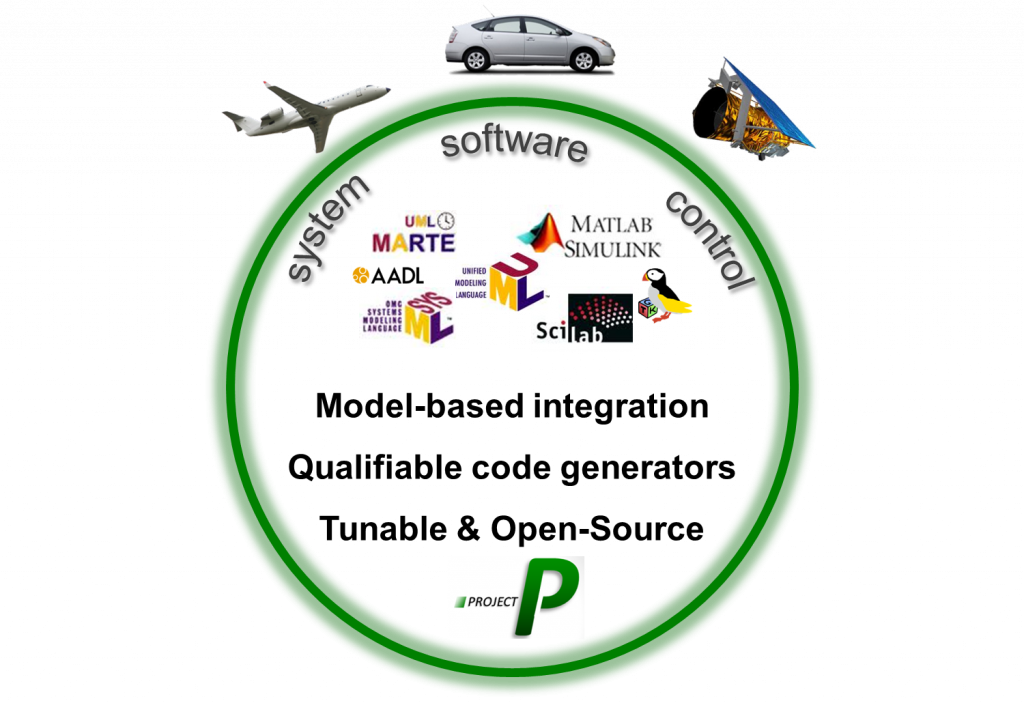
\includegraphics[scale=0.3]{images/projectp}
  \caption{Project P -- Source : {\tt http://www.open-do.org/projects/p/}}
  \label{fig:projectp}
\end{figure}

Parmi les collaborateurs de ce projet, on trouve de grands groupes industriels
(Airbus, Astrium, Continental, Rockwell Collins, Safran, Thales), des PME
(AdaCore, Altair, Scilab Enterprise, STI), des sociétés de services (ACG, Aboard
Engineering, Atos Origins) mais aussi des centres de recherche (CNRS, ENPC,
INRIA, ONERA).\\

AdaCore a ensuite développé un produit commercial à partir des
technologies développées dans Project P : QGen.

\begin{figure}[h]
  \centering
  
\includegraphics[scale=0.2]{images/qgen}
  \caption{QGen -- Source AdaCore}
  \label{fig:qgen}
\end{figure}

\section{Les outils de la plateforme}
La plateforme Orianne est développée en Java. Le projet est composé de plusieurs modules pour séparer les différents outils.
Deux principaux modules séparent la partie IHM qui sert à la configuration des outils d'une part et les générateurs de code d'autre part.
\subsection{La partie IHM}
La partie IHM s'organise sous forme d'onglets correspondant à la configuration de chaque outil (cf. figure \ref{fig:plateforme}). 
\begin{description}
  \item[Configuration moteur] Cette partie permet de configurer les éléments relatifs à un moteur. Le type de carburant, de combustion, d'injection, les fonctions à intégrer dans l'application finale.
  \item[Configuration fonctions] Chaque fonction cochée dans le premier onglet, peut être configurée dans le deuxième onglet. Les fonctions sont donc configurables via des éléments graphiques comme des cases à cocher, des champs texte ou des liste déroulantes.
  \item[Configuration RTOS] Cet onglet reprend les différences fonctions triées par leur récurrence sous forme de tableau. Chaque ligne représente un point d'entrée d'une fonction de contrôle moteur. L'ordre est significatif et peut être modifié via des boutons. L'ordre des fonctions dans cette table sera répercuté dans le fichier source de configuration du RTOS.
  \item[Configuration \gloss{ecu} \& \gloss{rte}] Cette section fait le lien entre les API fournies par les pilotes du calculateur moteur et les variables d'entrée/sortie des fonctions de l'application. En configurant les capteurs et actionneurs du calculateur avec leurs données (variables), la plateforme permet de faire la correspondance entre ces variables et les données consommées par les différentes fonctions de l'application.
  \item[Configuration CAN] L'ECU n'est pas le seul calculateur dans un véhicule. La communication entre ces différentes unités se fait généralement via un bus CAN. L'onglet CAN permet de configurer les différentes cellules de communication et accepte des fichiers XML représentant les différents messages à envoyer sur une cellule définie. L'interface permet également de faire correspondre les signaux reçus ou envoyés à des variables de l'application en entrée ou en sortie des fonctions.
\end{description}

\subsection{La partie génération}
L'interface de la plateforme a un menu regroupant les différentes actions de
génération possibles via la plateforme (cf figure \ref{fig:toolsMenu}).
\begin{description}
  \item[Génération CAN] Cette action crée deux fichiers source {\tt.c} et {\tt
	.h} reprenant la configuration de la communication CAN.
  \item[Génération RTOS] Cette action reprend les listes des points d'entrée des
	modules de l'application en fonction de leur place dans la configuration.
  \item[Génération RTE] Cette action crée deux fichiers source {\tt.c} et {\tt
	.h} déclarant l'ensemble des entrées/sorties des fonctions qui seront
	échangées entre les différents modules. Elle génère aussi les fonctions
	d'accès en lecture et en écriture des données fournies par le matériel du
	calculateur moteur par l'intermédiaire de pilotes.
  \item[Génération Orianne] Cette action met en place les fichiers aux
	emplacements requis pour la compilation d'une application complète. Elle
	copie les sources générées par la plateforme et celles importées depuis la
	génération de code des modèles Simulink\up{\circledR}.
  \item[Compilation] Cette action lance la compilation d'une application
	complète via le compilateur défini dans la configuration de la plateforme.
  \item[Génération \gloss{a2l}] Cette action génère le fichier A2L servant de
	dictionnaire des variables dans la mémoire du calculateur.
\end{description}

\begin{figure}[h]
  \centering
  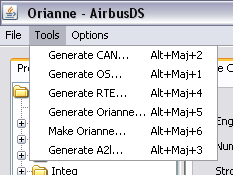
\includegraphics[scale=0.7]{images/toolsMenu}
  \caption{Plateforme Orianne, menu Tools (capture du 17 juin 2015)}
  \label{fig:toolsMenu}
\end{figure}

\subsection{La problématique}
La problématique autour de cette plateforme est simple : tous les outils ne sont
pas encore créés.

Afin que la plateforme garde une certaine stabilité, les générateurs non
implémentés sont remplacés par une simple copie de fichiers génériques embarqués
en dur dans la plateforme. Ces fichiers doivent ensuite être modifiés à la main
pour correspondre aux besoins de l'application conçue via la plateforme. Ainsi,
les fichiers sont en place pour faciliter la compilation d'une application.
L'utilisateur n'a alors plus qu'à modifier les fichiers dont il a besoin et
lancer la compilation.

Parmi les outils manquant à la plateforme, je vais me concentrer sur la
génération CAN et la génération RTE, les outils sur lesquels j'ai travaillé. Il
faudra donc développer les interfaces graphiques et les générateur
correspondants. La prise en compte de ces nouveaux outils aura un impact sur les
autres outils comme par exemple la génération RTOS qui devra prendre en compte
les nouveaux points d'entrée de la communication CAN dont la structure pourra
changer pas rapport à leur ancienne version.

\begin{figure}[h]
  \centering
  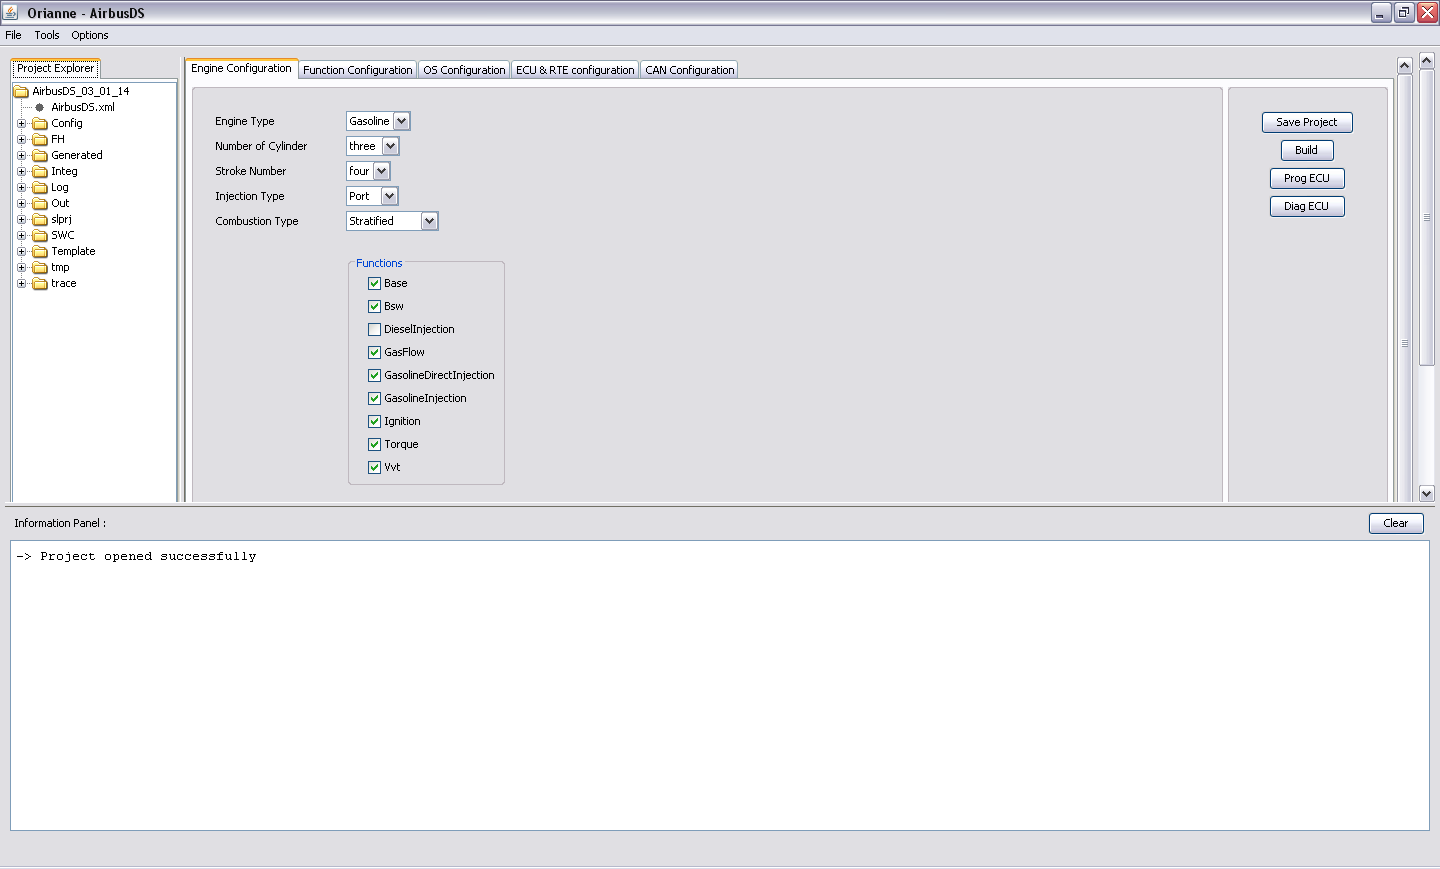
\includegraphics[angle=-90, scale=0.5]{images/plateforme}
  \caption{Plateforme Orianne, configuration moteur (capture du 17 juin 2015)}
  \label{fig:plateforme}
\end{figure}

